%! Author = lili
%! Date = 4/27/26

\section{Begrifflichkeiten}
\defin{Vererbung}
\defin{Variabilität}
\defin{Genetik}
\defin{asexFort}
\defin{sexFort}

\section{Chromosomen}
\defin{Karyotyp}
\frage{menschchromosomen}

\begin{figure}[H]
    % TODO Bild 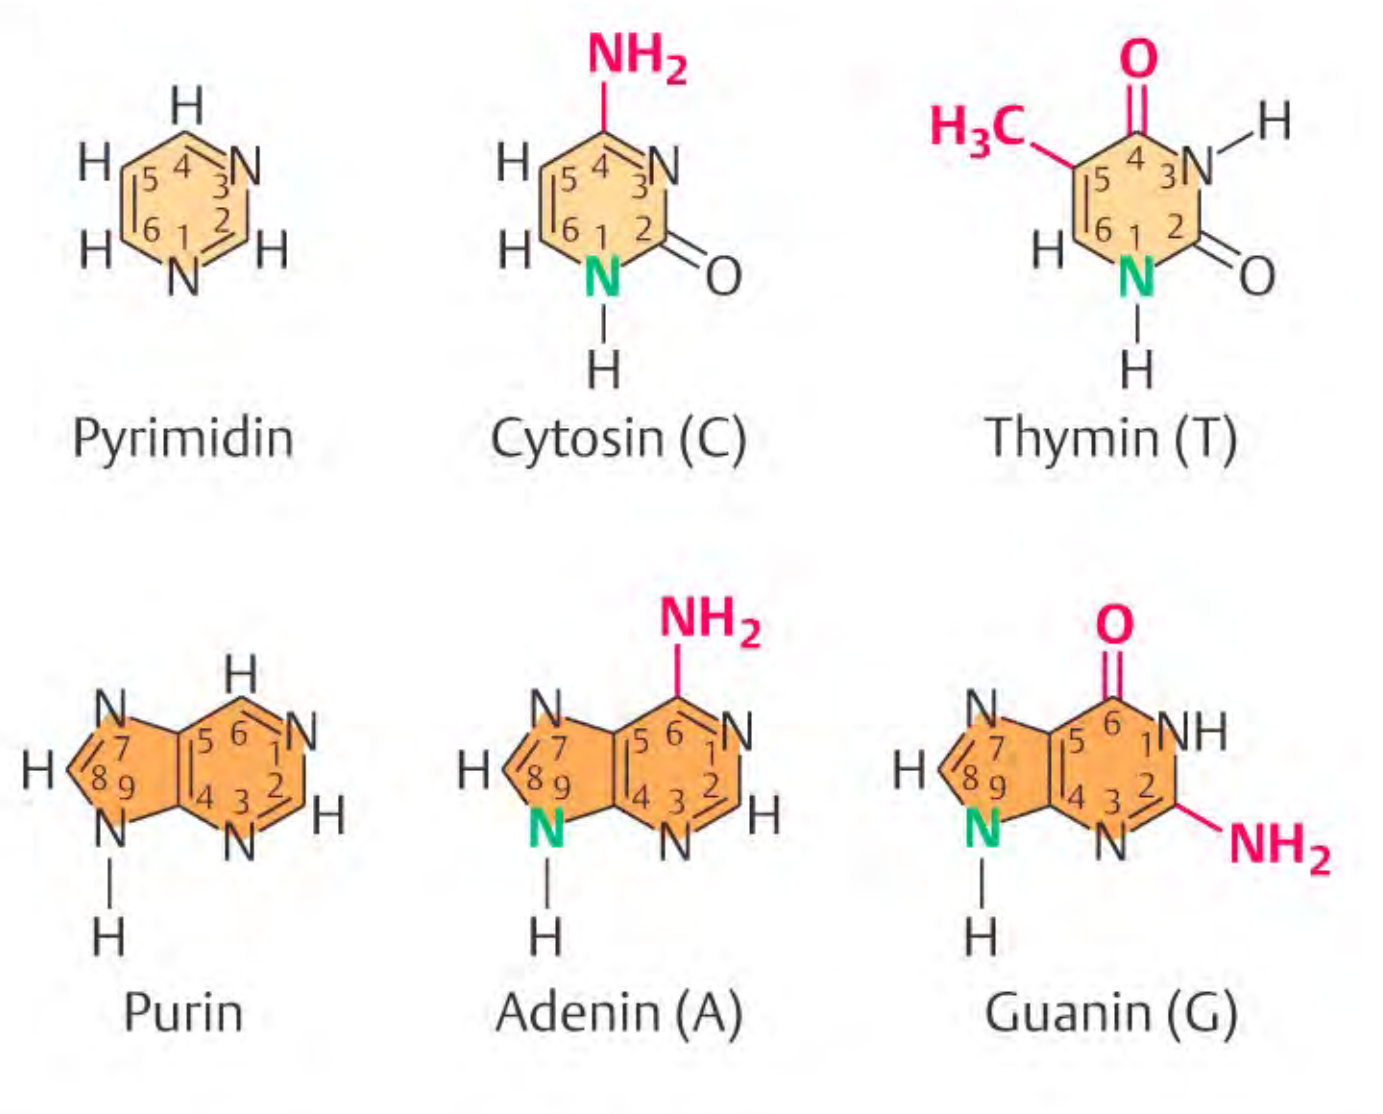
\includegraphics[width=\textwidth]{bilder/basen}
    \caption{Abbildung eines Mataphase-Chromosoms.}\label{fig:figure}
    % TODO Bildverdeckung
\end{figure}

\defin{Telomer}
\defin{Centromer}
\defin{Kinetochor}
\defin{Mikrotubuli}
\defin{Chromatid}

% TODO warum Farbkörperchen im Zellkern

\begin{figure}[H]
    % TODO Bild 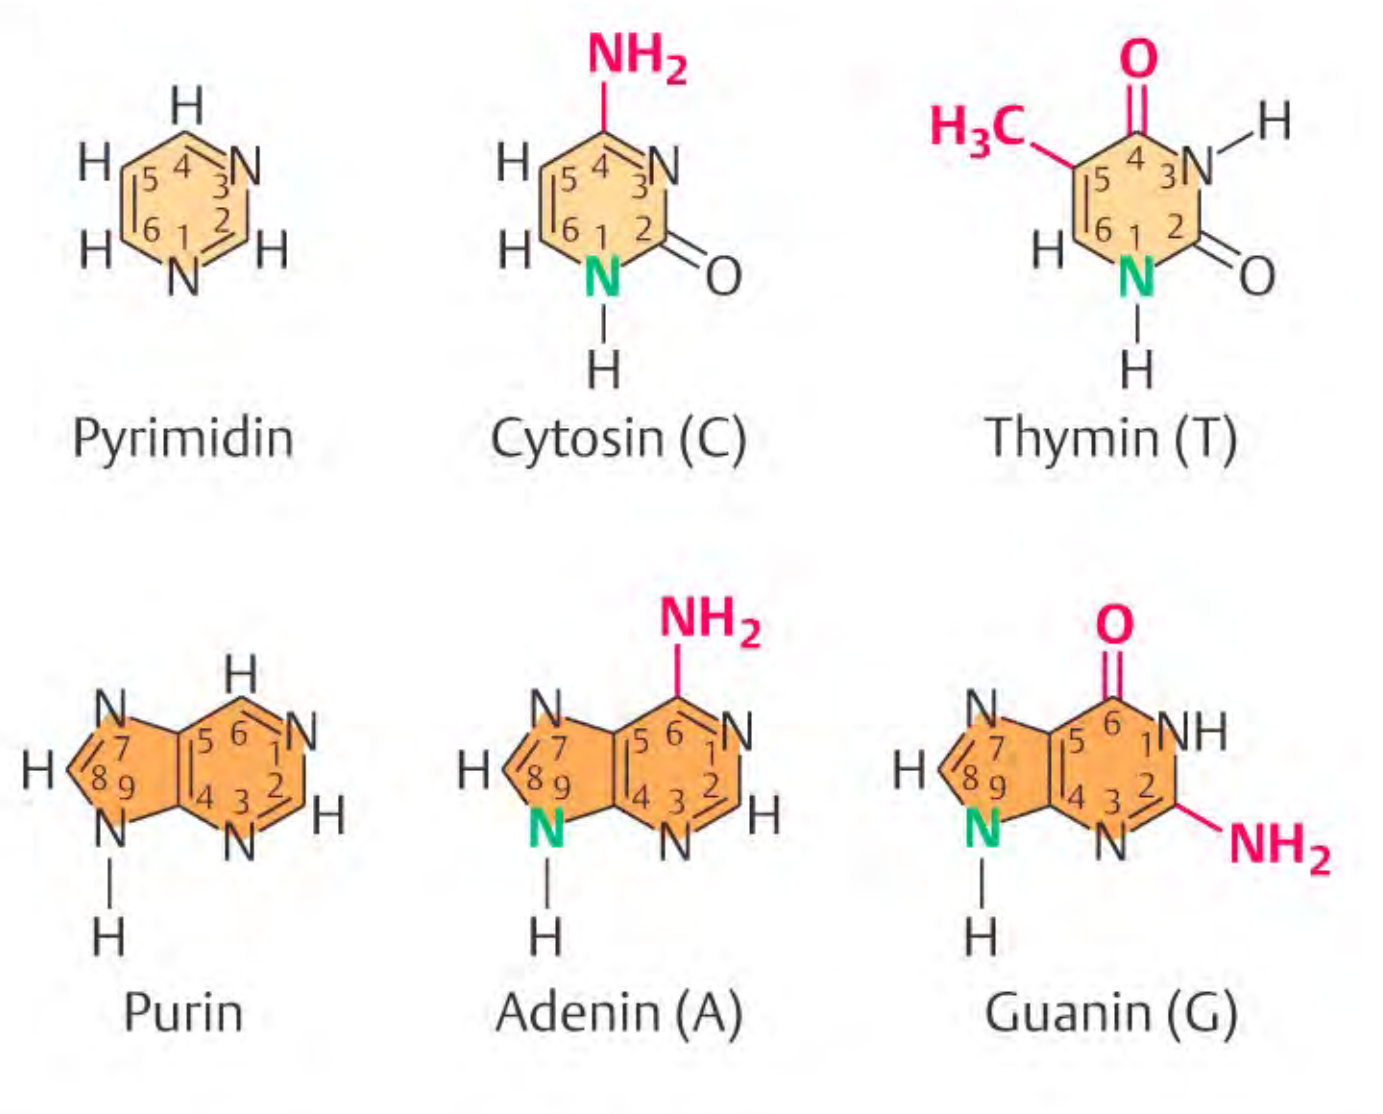
\includegraphics[width=\textwidth]{bilder/basen}
    \caption{Verschiedene Chromatin-Bereiche im Chromosom.}\label{fig:figure}
    % TODO Bildverdeckung
\end{figure}
\frage{wenigac}
\defin{Cohesin}

\subsection{Chromosomen-Kondensation}
Für die Kondensation der Chromatiden sind Condensin-Proteinkomplexe notwendig.
% TODO genauere Erklärung, evtl Bild F 22



\subsection{Chromosomensätze}

\defin{diploid}
\defin{haploid}

\frage{chromosomenzahlMensch}
\frage{nMensch}

\subsection{Schwesterchromosomen}

\defin{Schwesterchromosom}

\frage{washältzsm}

\begin{figure}[H]
    % TODO Bild 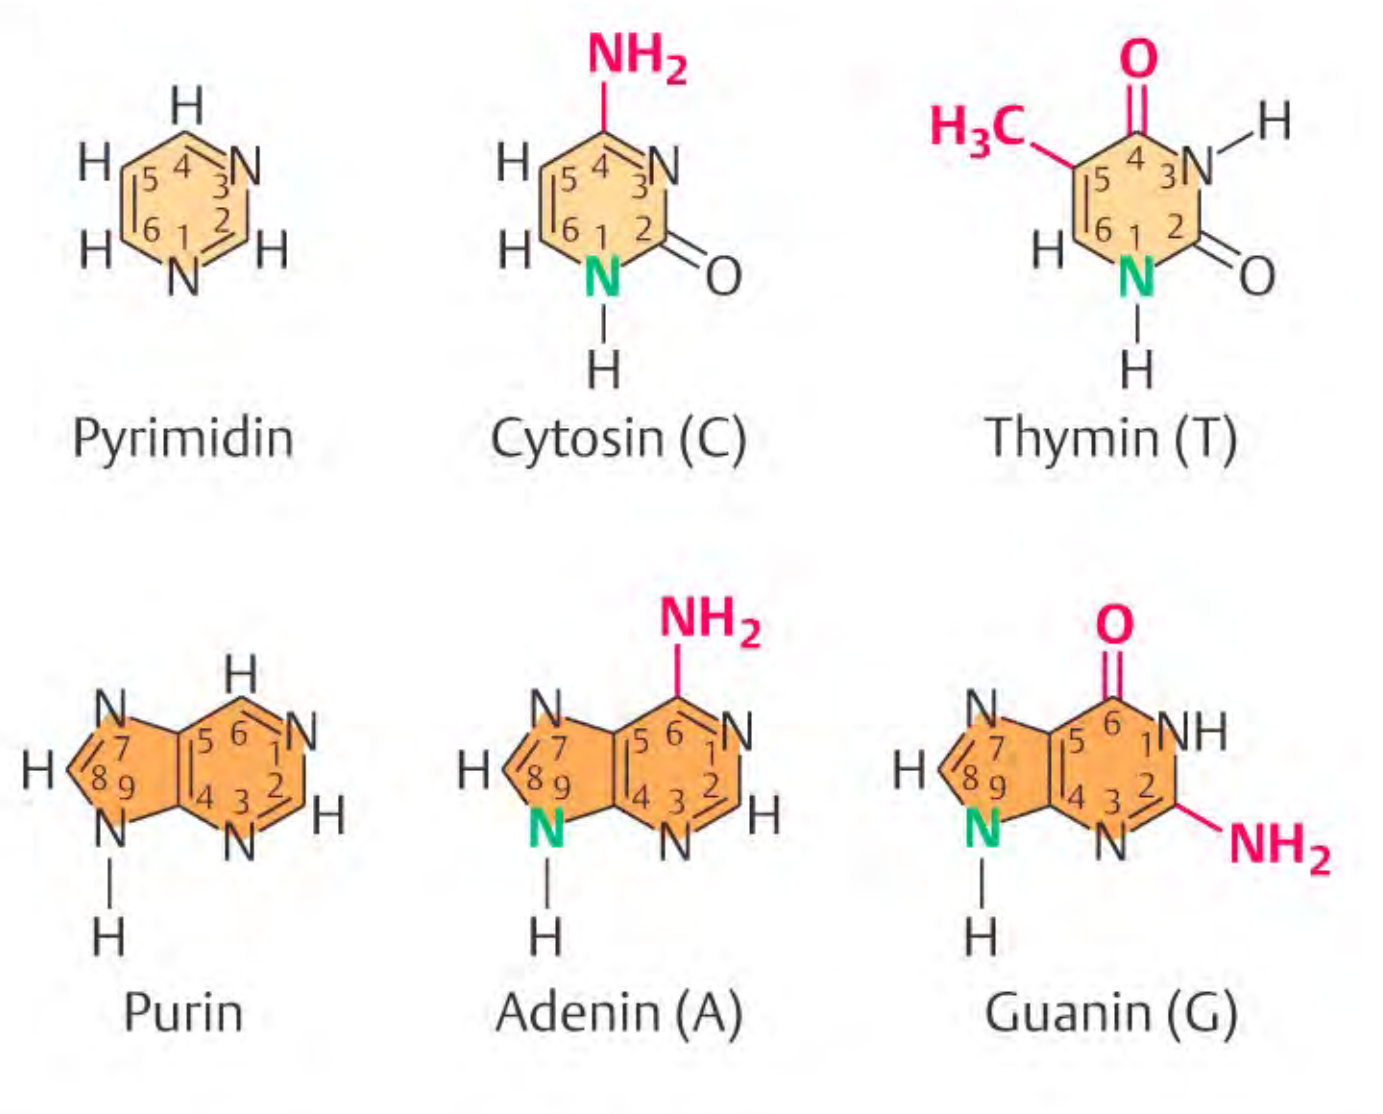
\includegraphics[width=\textwidth]{bilder/basen} F 26
    % TODO Bild 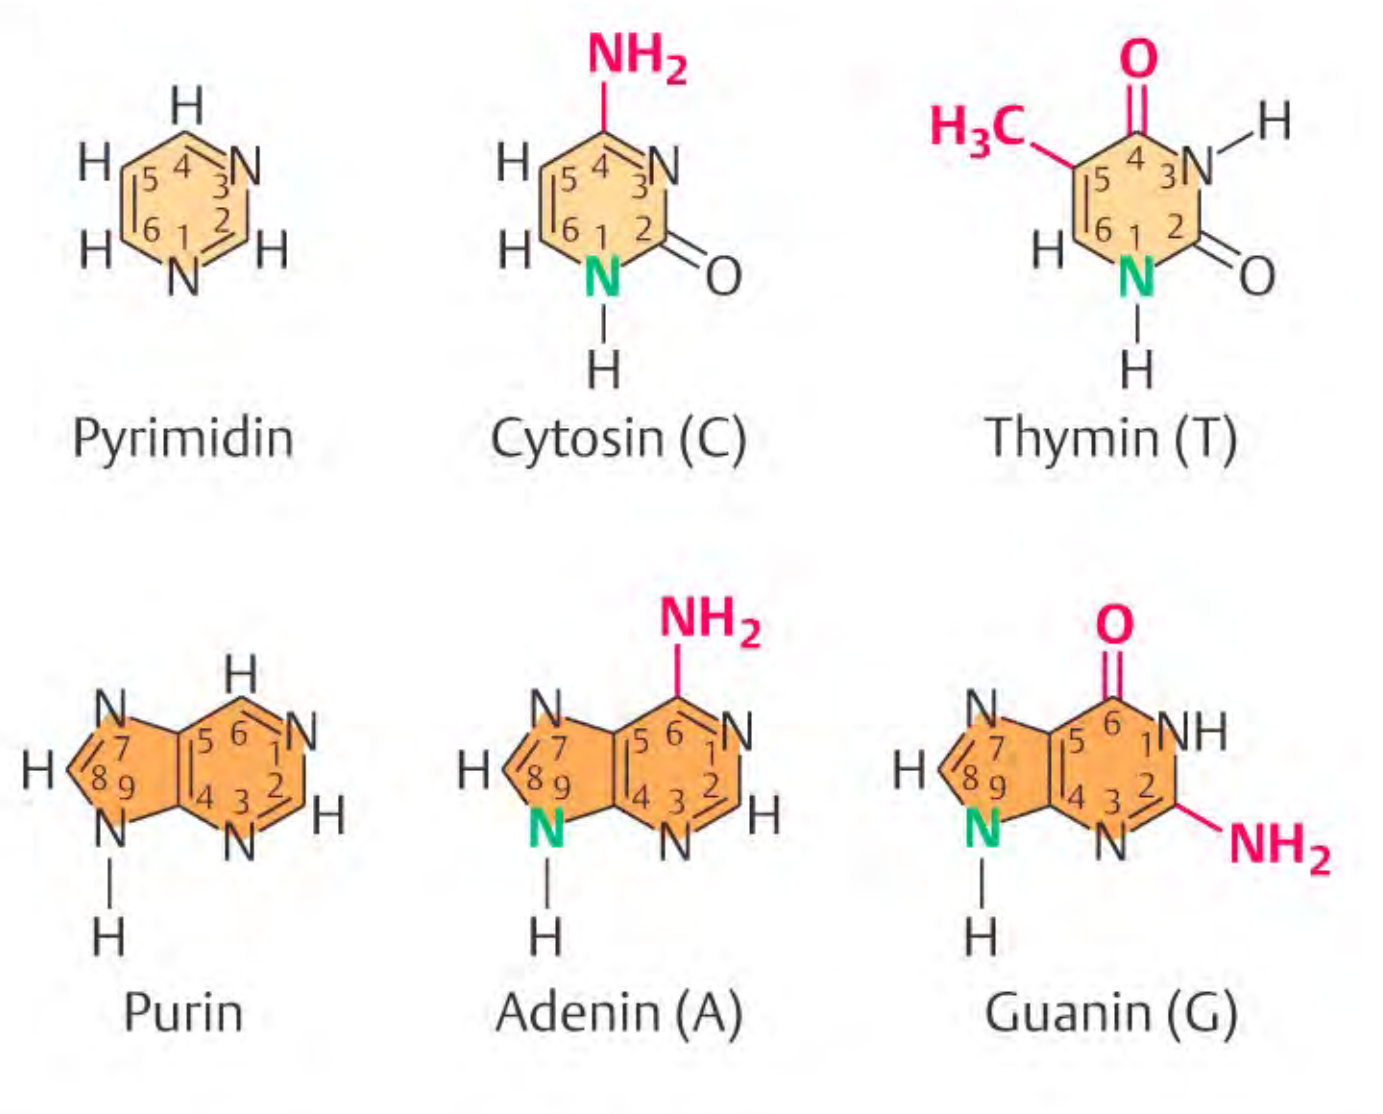
\includegraphics[width=\textwidth]{bilder/basen} F 27
    \caption{Verschiedene Darstellungsformen des Cohäsins.}\label{fig:figure}
\end{figure}
\section{Zellzyklus und Zellteilung}

\begin{figure}[H]
    \begin{subfigure}[t]{0.45\textwidth}
        \centering
        % TODO Bild 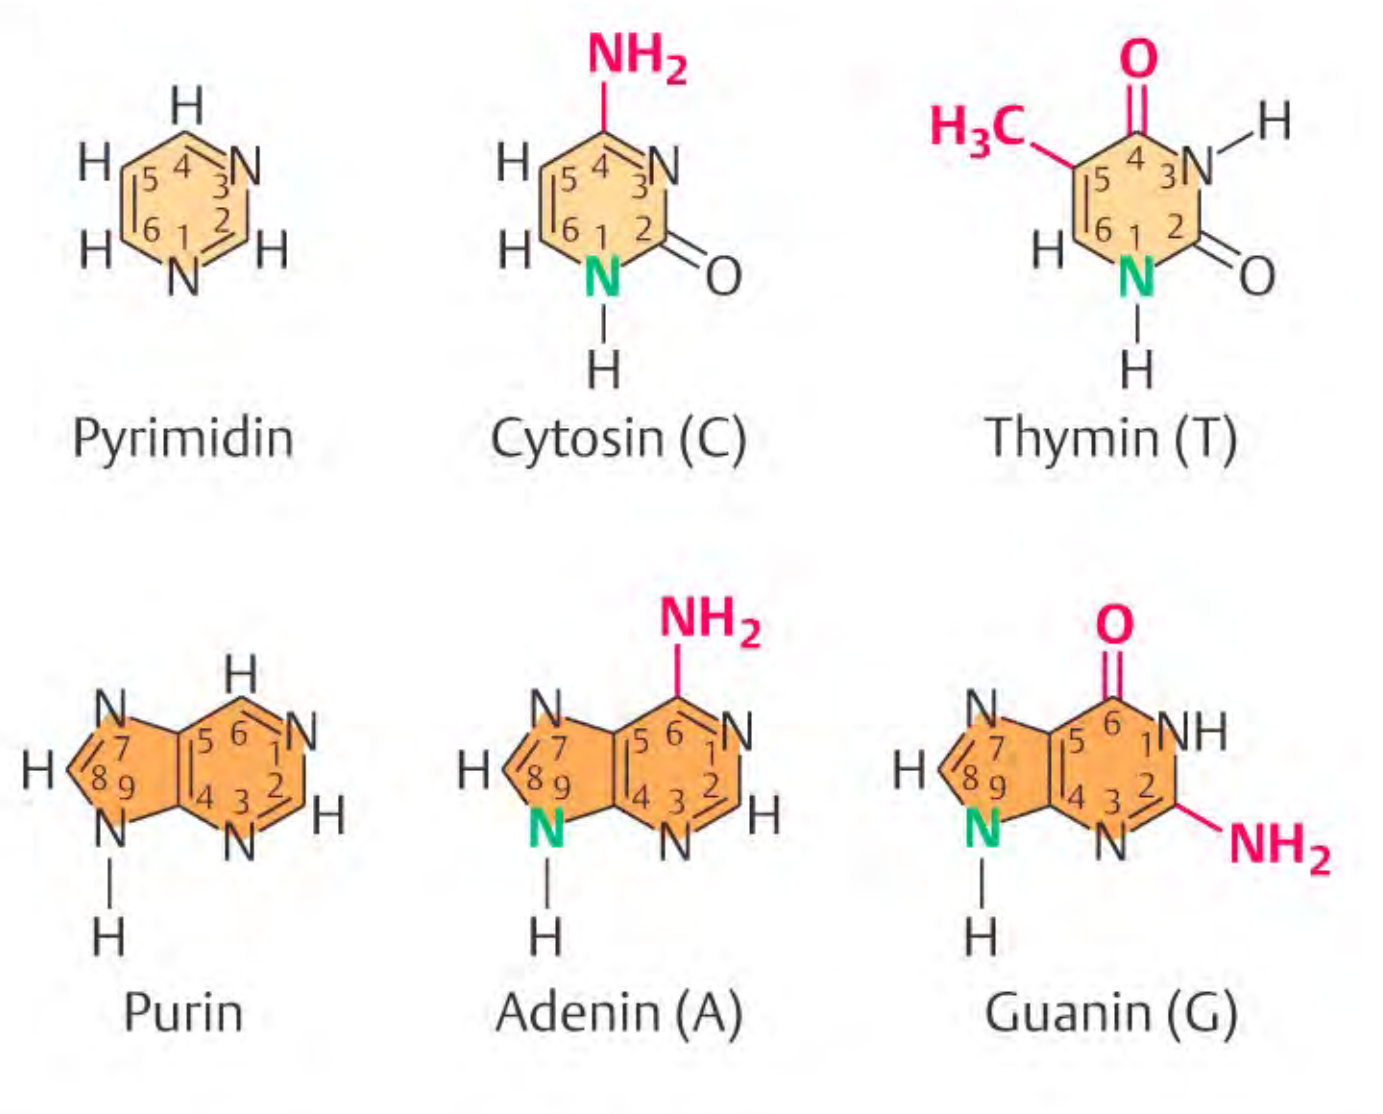
\includegraphics[width=\textwidth]{bilder/basen}
        % TODO Bildverdeckung
        \caption{Mit Fokus auf die Zellteilung.}\label{fig:figure}
    \end{subfigure}
    \hfill
    \begin{subfigure}[t]{0.45\textwidth}
        \centering
        % TODO Bild 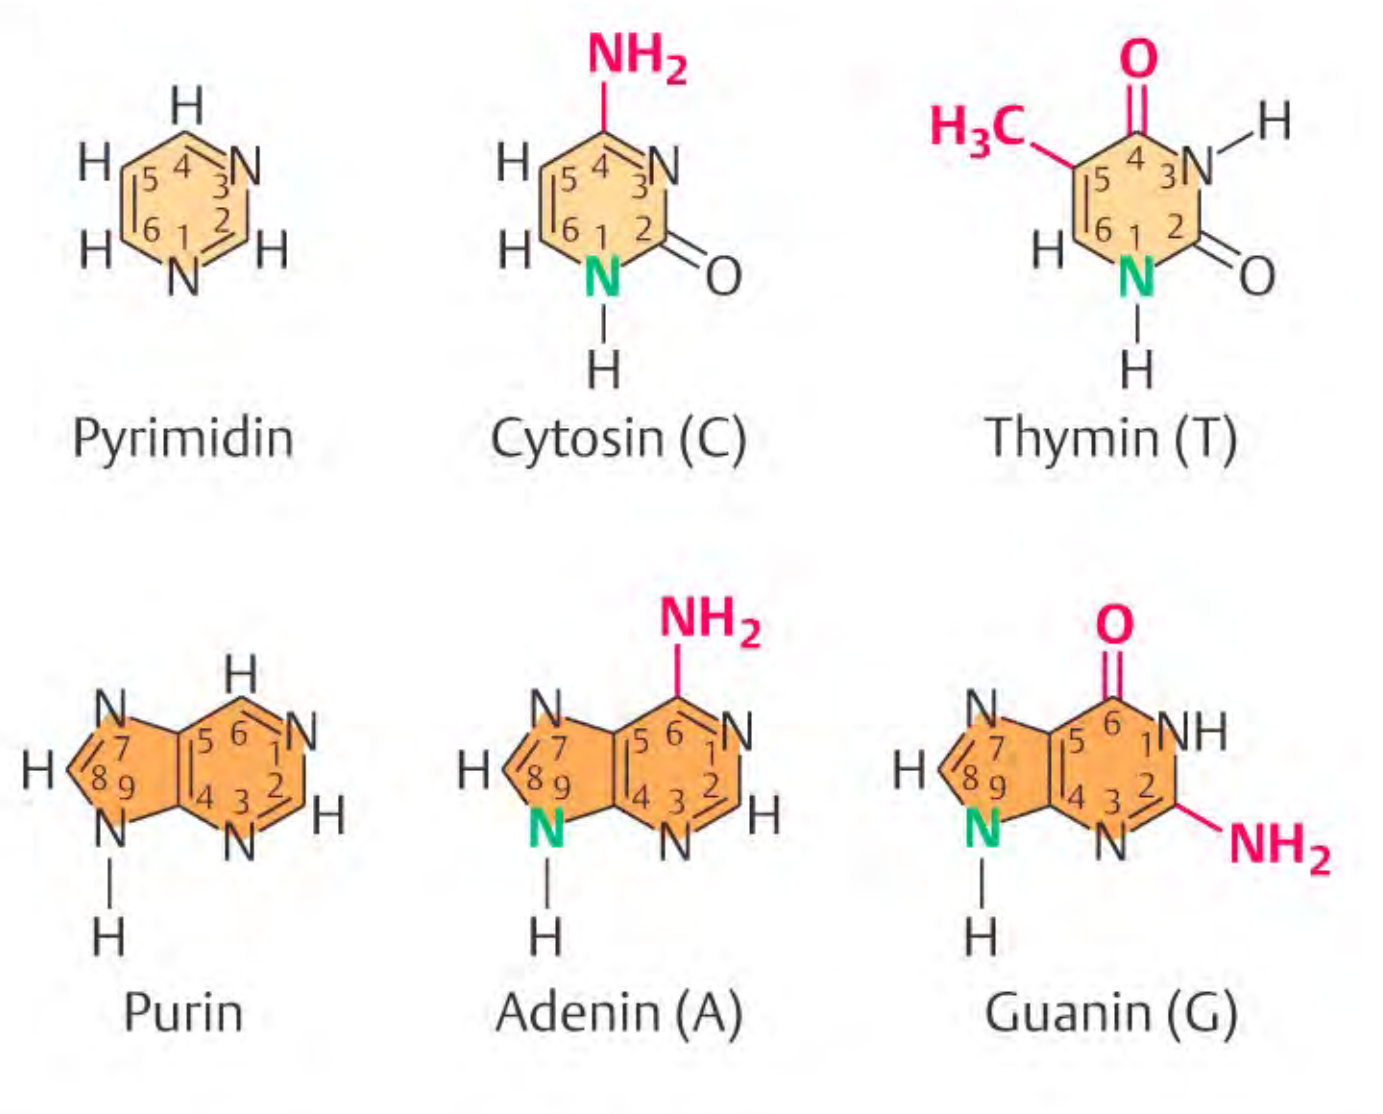
\includegraphics[width=\textwidth]{bilder/basen}
        % TODO Bildverdeckung
        \caption{Mit Fokus auf die Chromosomen.}\label{fig:figure}
    \end{subfigure}
    \caption{Verschiedene Betrachtungsweisen des Zellzyklus.}\label{fig:figure}
\end{figure}


\begin{figure}[H]
    % TODO Bild 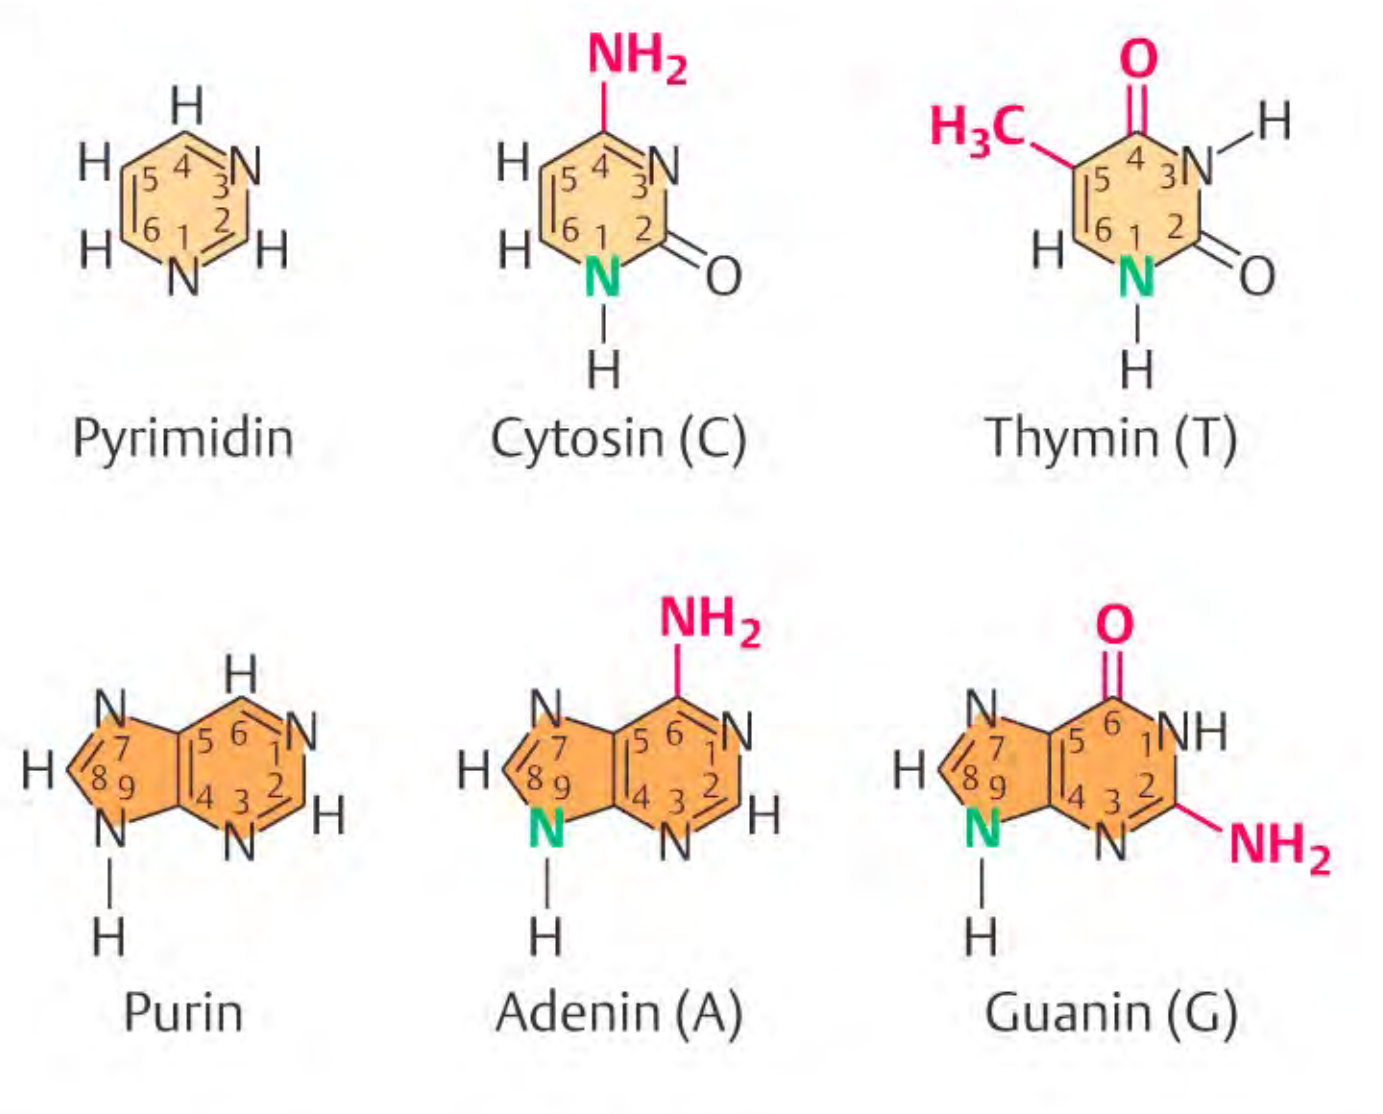
\includegraphics[width=\textwidth]{bilder/basen} F 20
    \caption{Menge an DNA, RNA und Proteinen im Verlauf des Zellzyklus.}\label{fig:figure}
\end{figure}

\frage{wannchromo}

\subsection{Mitose}
\frage{wasinmitose}

\frage{ausnahmeMitose}
Sonst würde ja mit jeder Generation der Chromosomensatz verdoppelt!

\subsubsection*{Die Phasen der Mitose}

\begin{figure}[H]
        % TODO Bild 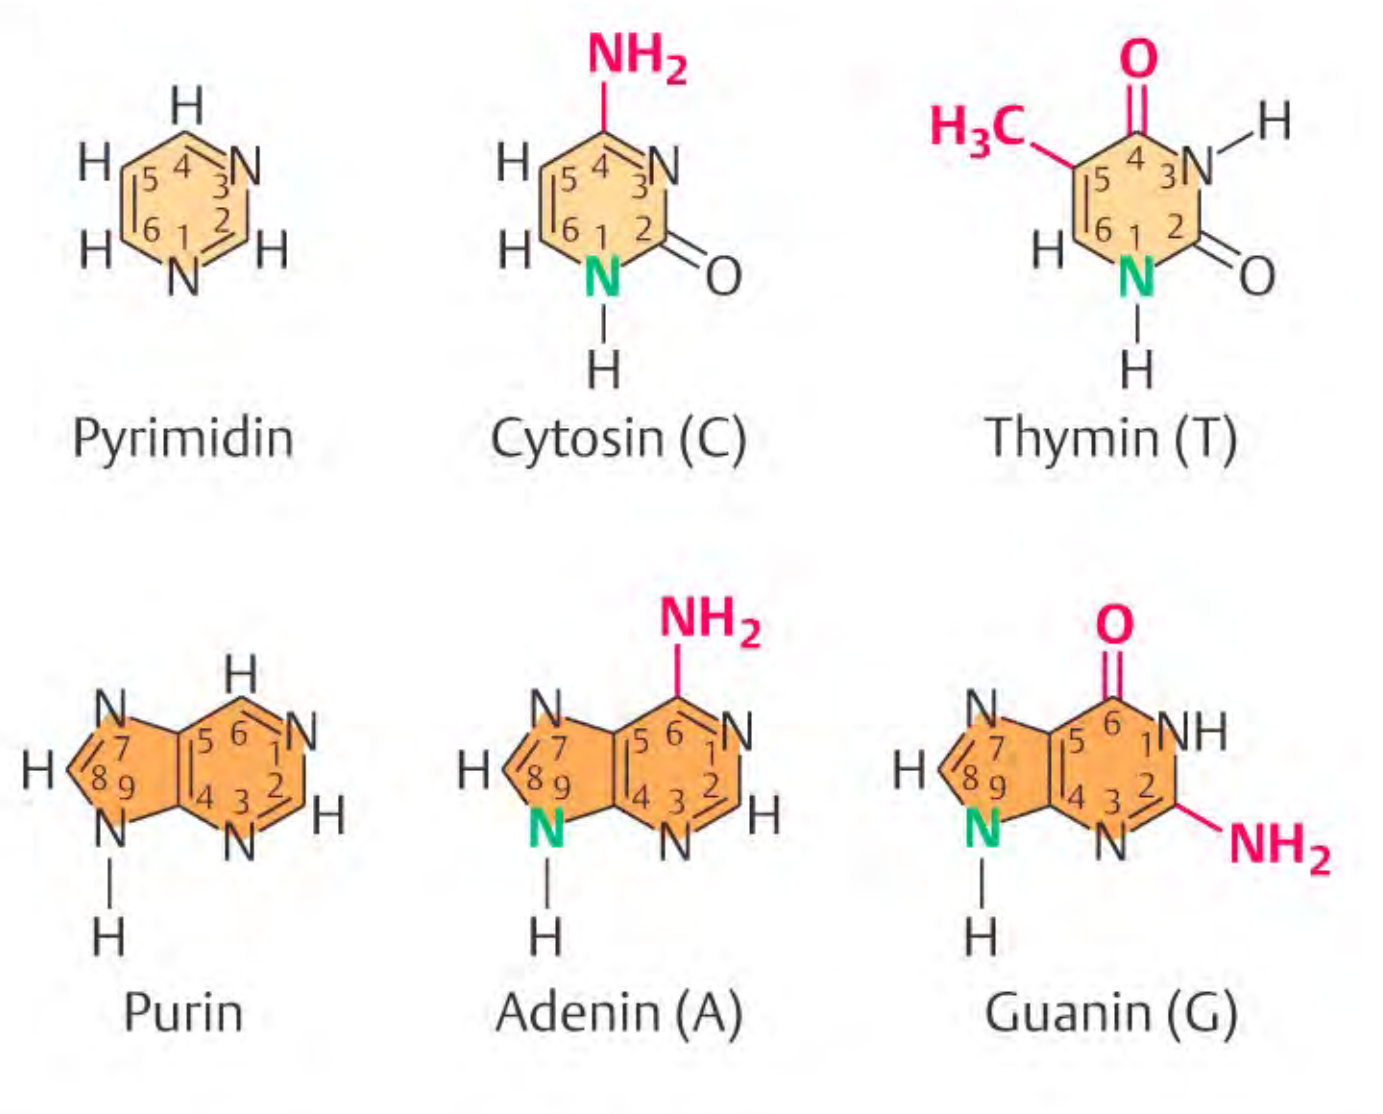
\includegraphics[width=\textwidth]{bilder/basen} F 24
    \caption{Die Phasen der Mitose und die Form des Chromatins.}\label{fig:figure}
\end{figure}

\frage{wiechromg1}
\frage{wiechromg2}
\frage{wiechrommetaphase}

%todo folie 25

\subsection{Entwicklungszyklen}
\defin{Haplont}
\defin{Diplont}
\defin{Diplohaplont}

\begin{figure}[H]
    % TODO Bild 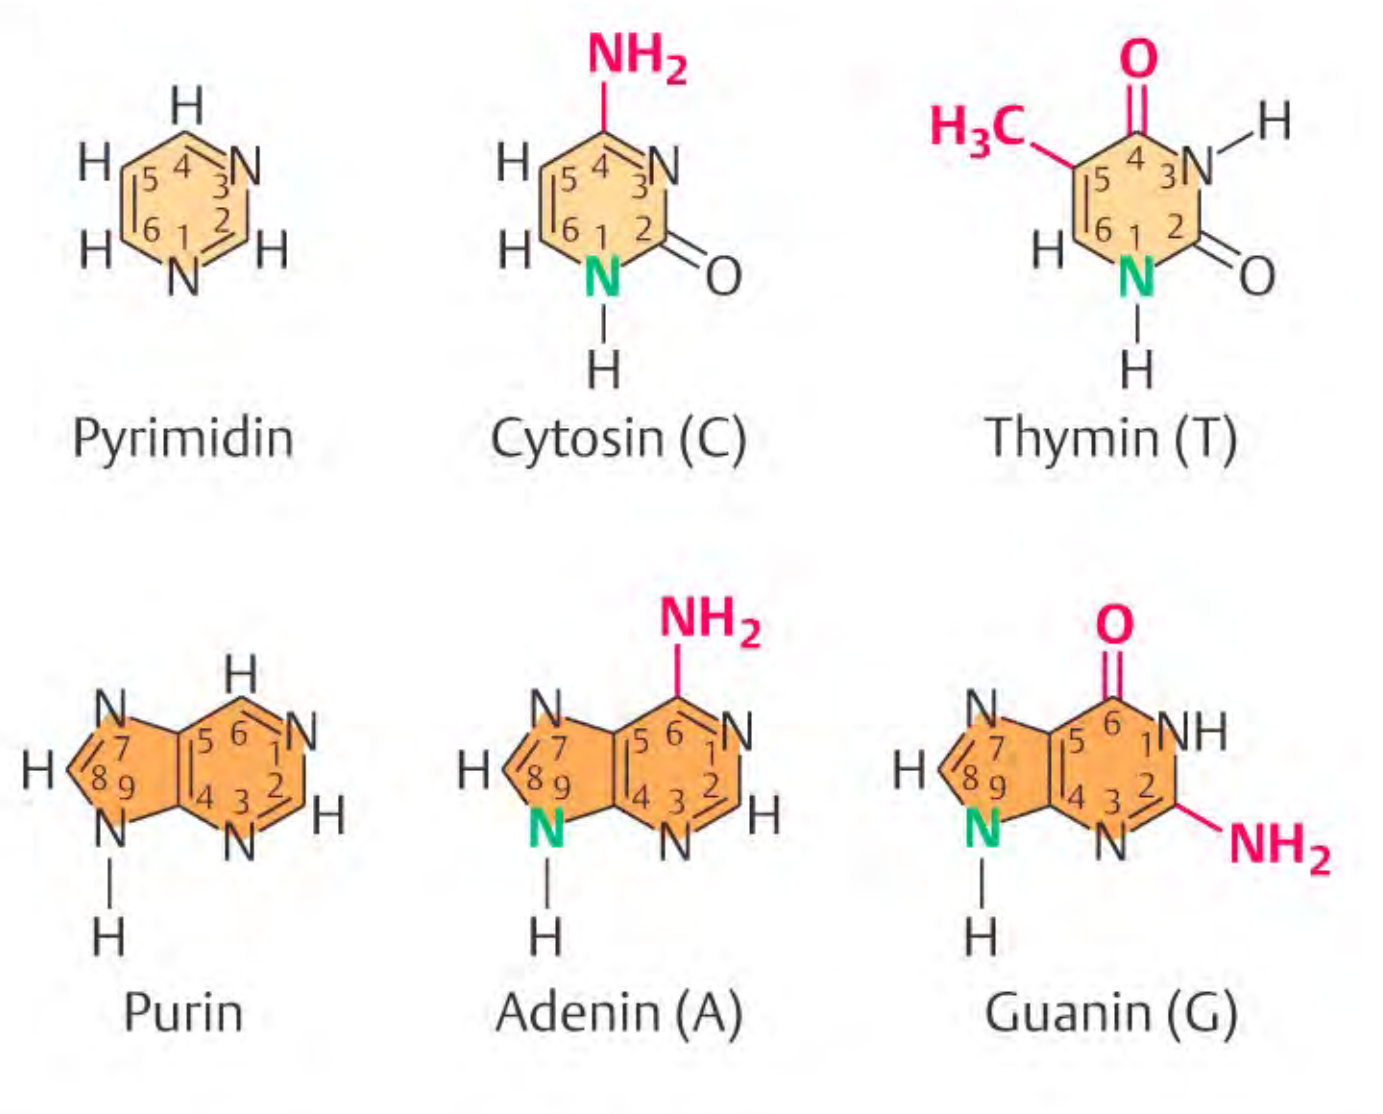
\includegraphics[width=\textwidth]{bilder/basen} F 29-37
    \caption{Die Phasen der Mitose und die Form des Chromatins.}\label{fig:figure}
\end{figure}

\begin{figure}[H]
    % TODO Bild 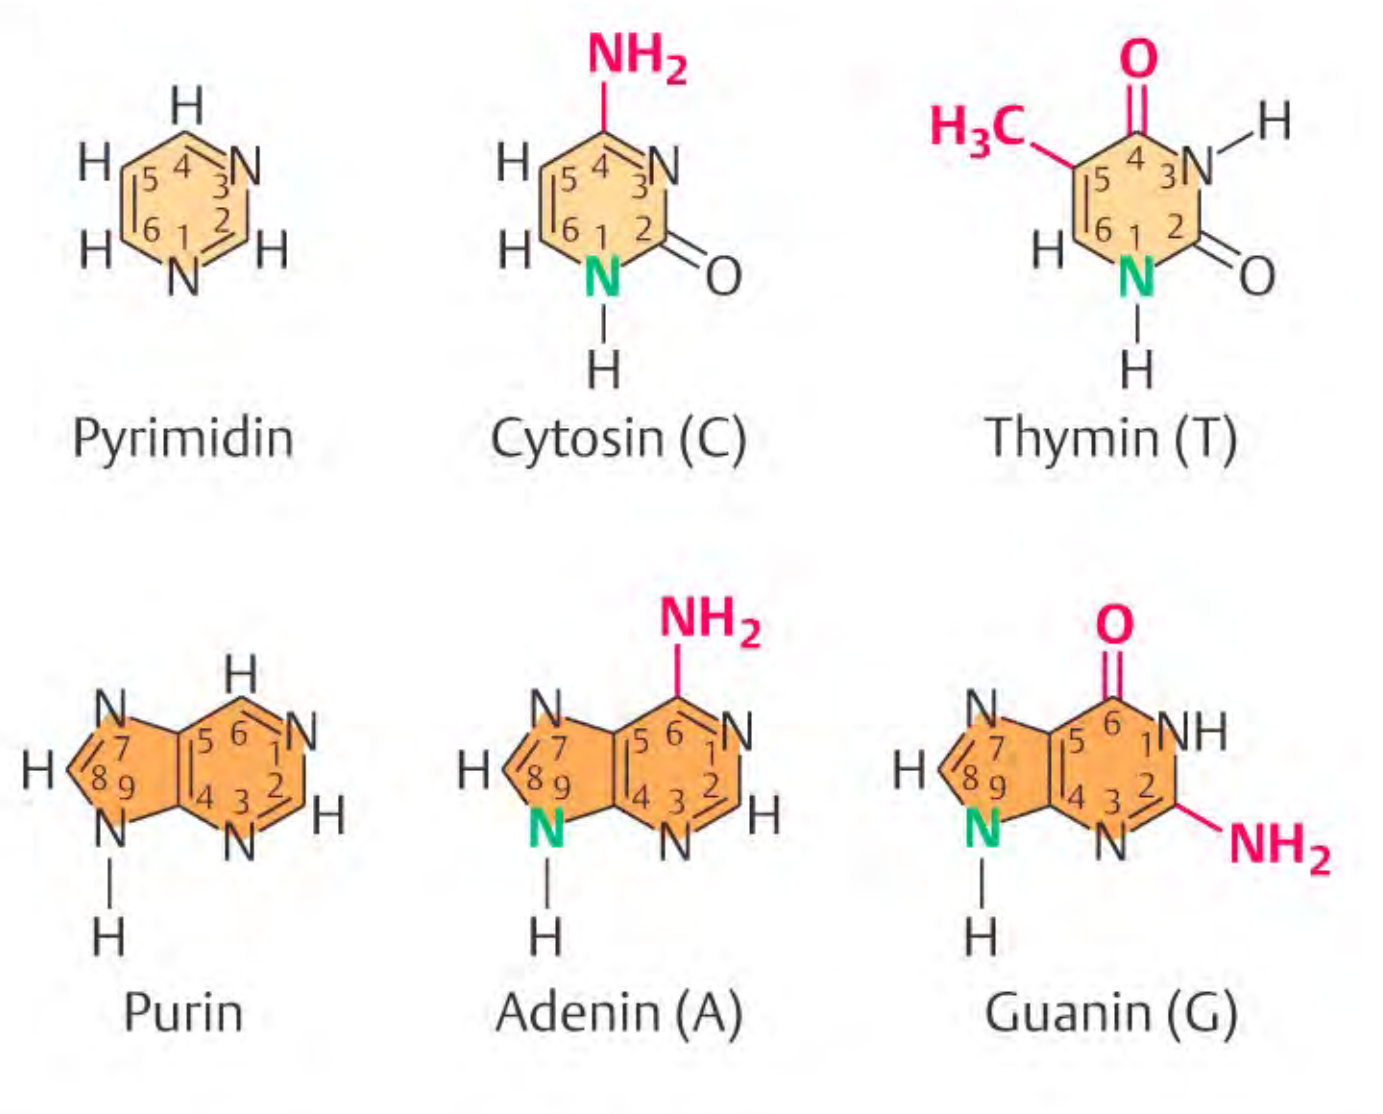
\includegraphics[width=\textwidth]{bilder/basen} F 29-31
    \caption{Entwicklungszyklus in Tieren.}\label{fig:figure}
\end{figure}

\begin{figure}[H]
    % TODO Bild 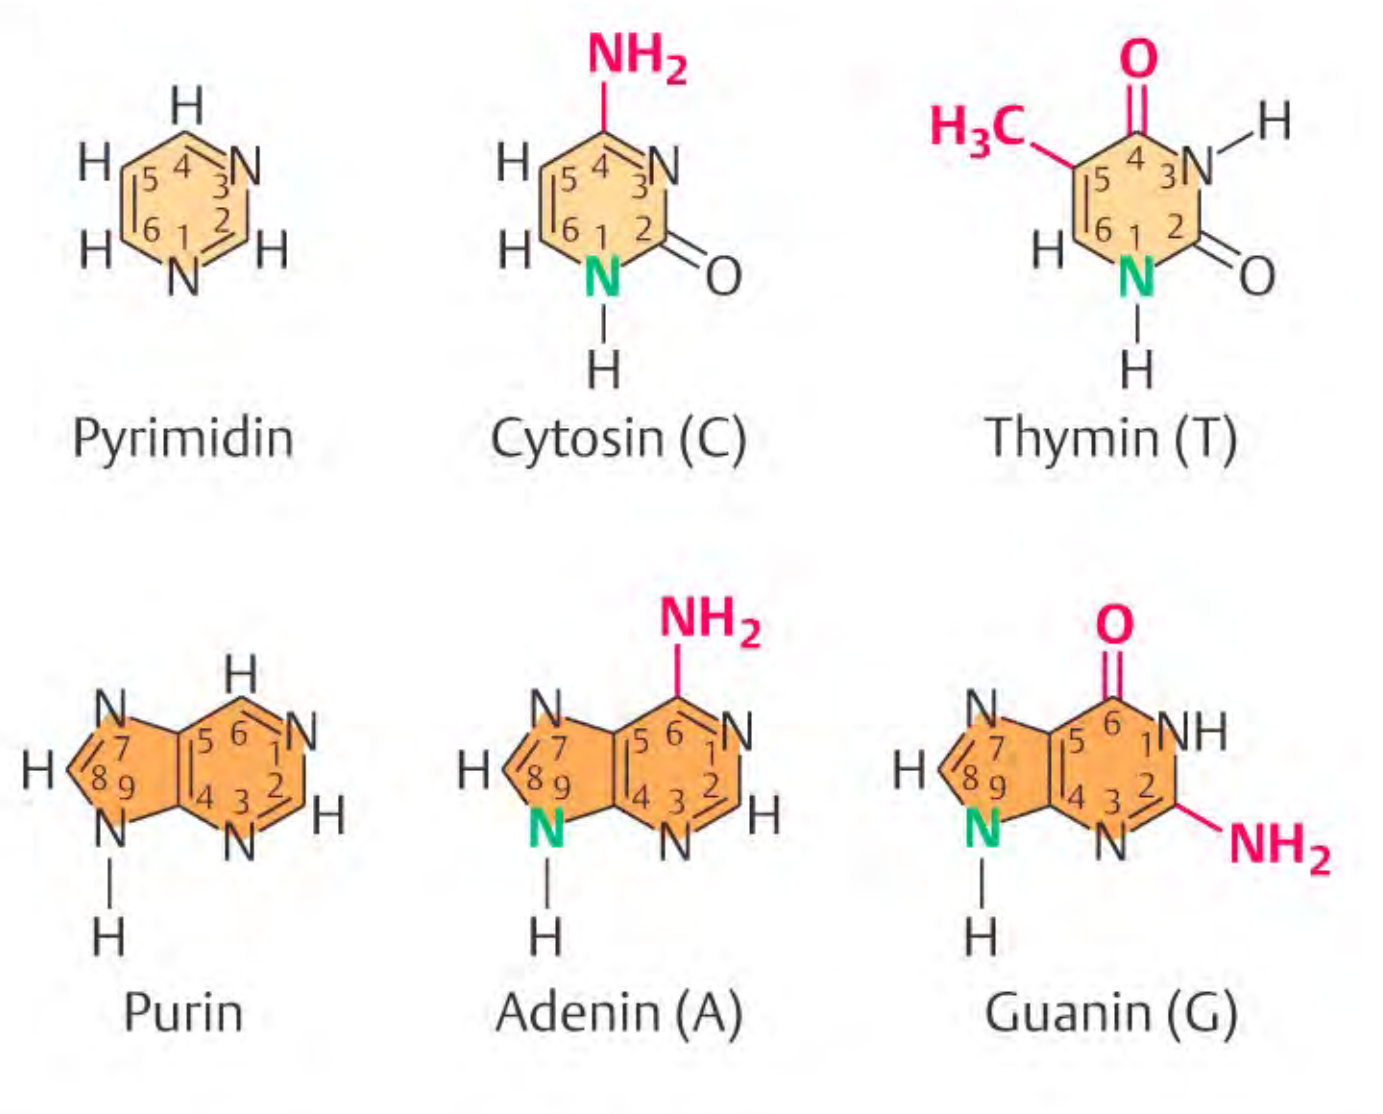
\includegraphics[width=\textwidth]{bilder/basen} F 32-34
    \caption{Entwicklungszyklus in haploiden vielzelligen Organismen.}\label{fig:figure}
\end{figure}


\begin{figure}[H]
    % TODO Bild 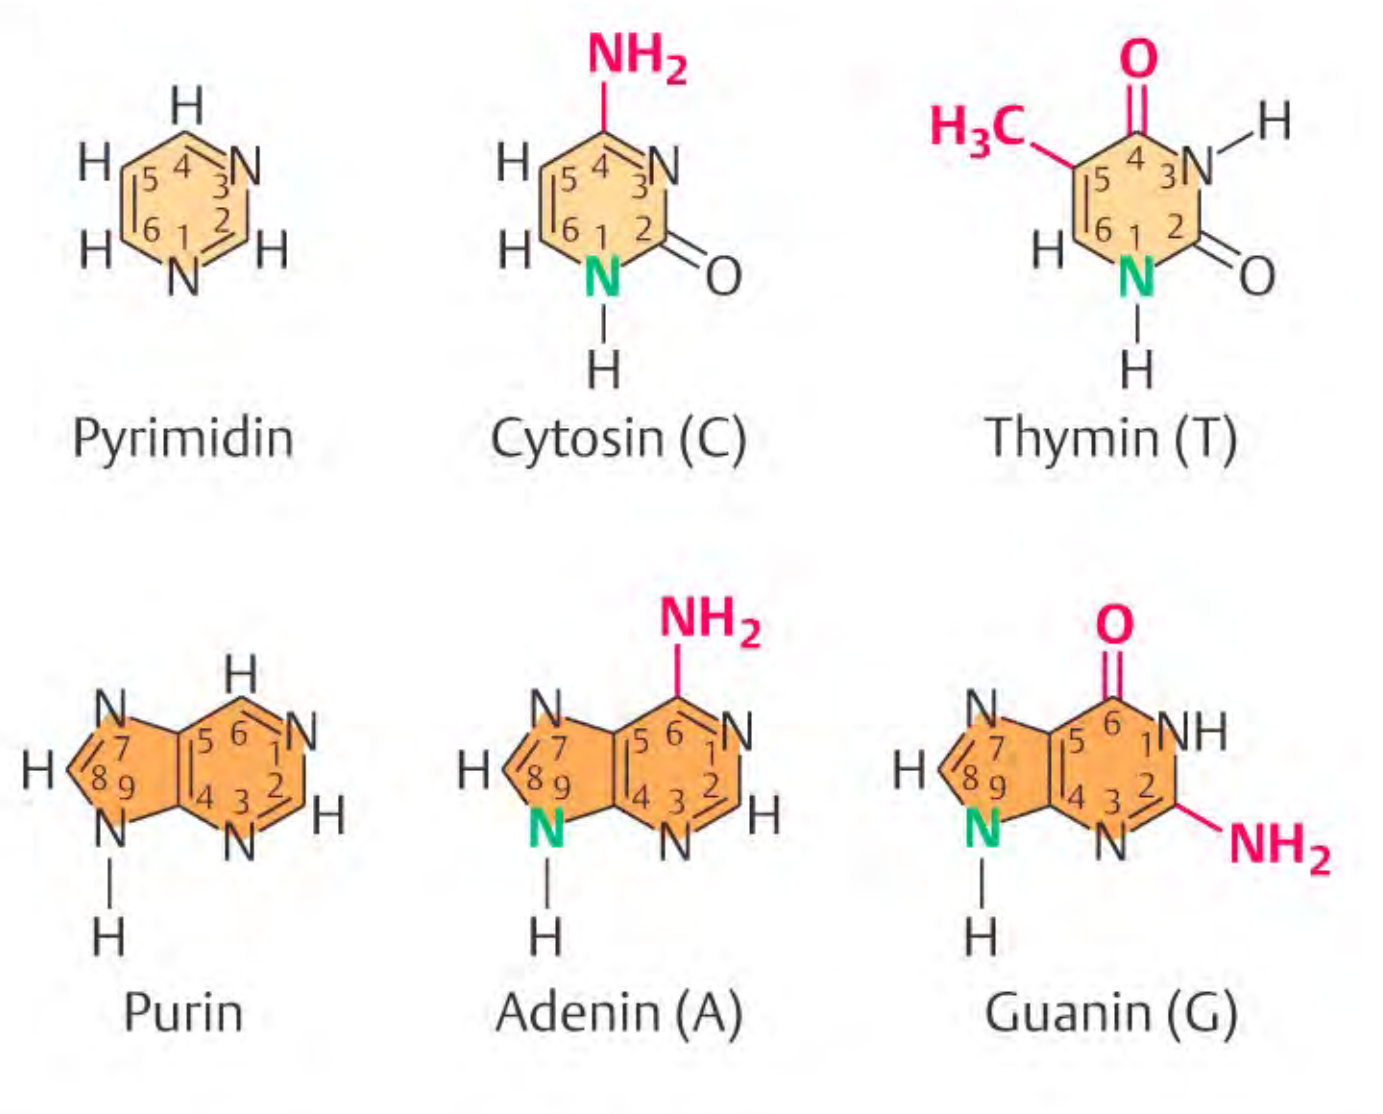
\includegraphics[width=\textwidth]{bilder/basen} F 35-37
    \caption{Weiterer Entwicklungszyklus in haploiden vielzelligen Organismen (Diplohaplonten).}\label{fig:figure}
\end{figure}


\begin{figure}[H]
    % TODO Bild 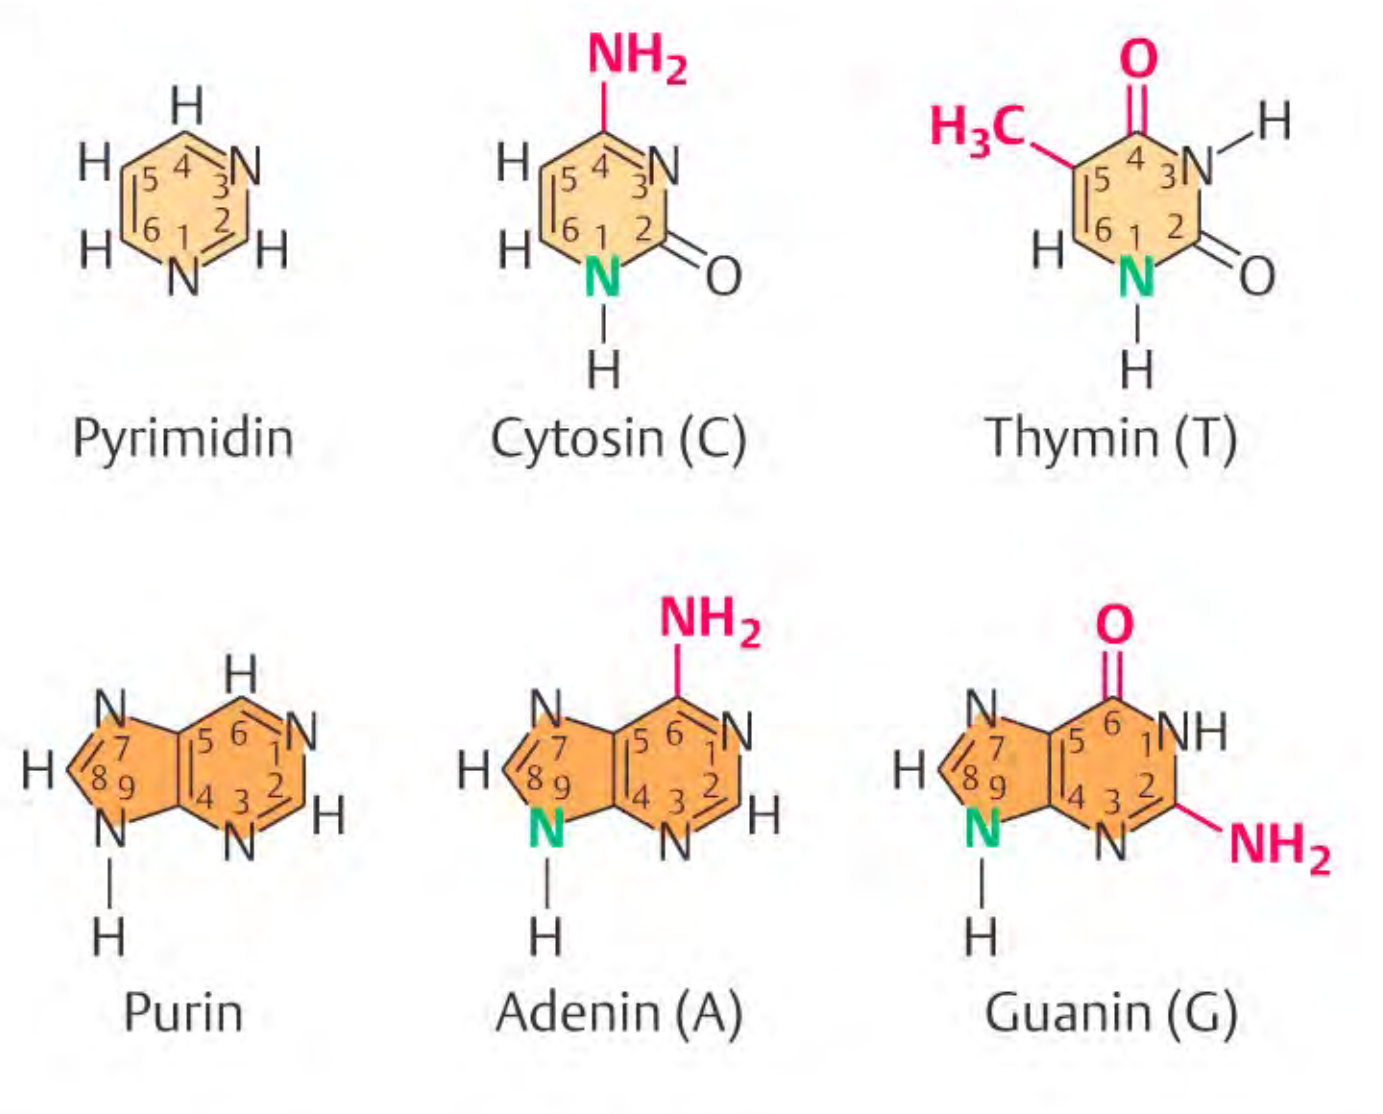
\includegraphics[width=\textwidth]{bilder/basen} F 39
    \caption{Vergleich der Entwicklungszyklen von Haplonten, Diplonten und Diplohaplonten.}\label{fig:figure}
\end{figure}



\subsection{Meiose}

Die Meiose ist eine sog. \gls{Reduktionsteilung}.

\defin{Reduktionsteilung}


% kam bis folie 39